\documentclass[twocolumn,superscriptaddress,aps]{revtex4-1}


%%%%%%%%%%%%
% Packages %
%%%%%%%%%%%%

\usepackage[utf8]{inputenc}

\usepackage{amsfonts}
\usepackage{amssymb}
\usepackage{amsmath}
\usepackage{amsthm}

\usepackage{bbold}
\usepackage{bm}
\usepackage{graphicx}
\usepackage{color}
\usepackage{hyperref}


%%%%%%%%%%%%
% Document %
%%%%%%%%%%%%

\begin{document}
    % ----- Title ----- %
    
    \title{\Large{INFO8010 : Neural style transfer}}
    \vspace{1cm}
    
    \author{\small{\bf Maxime Meurisse}}
    \affiliation{\texttt{m.meurisse@student.uliege.be} (\texttt{s161278})}
    
    \author{\small{\bf Adrien Schoffeniels}}
    \affiliation{\texttt{adrien.schoffeniels@student.uliege.be} (\texttt{s162843})}
    
    \author{\small{\bf Valentin Vermeylen}}
    \affiliation{\texttt{valentin.vermeylen@student.uliege.be} (\texttt{s162864})}
    
    \maketitle
    
    %%%%%%%%%%%%%%%%%%%%
    %%%%%%%%%%%%%%%%%%%%
    %%%%%%%%%%%%%%%%%%%%
    
    % ----- Introduction ----- %
    
    % TO DO
    % -----
    % States the problem which has been tackled
    
    \section{Introduction}
    
    We have decided to tackle the task of \emph{neural style transfer}. The goal of such a task is to combine the content and style of two different images.\\
    
    An example of is provided at Figure \ref{fig:example}.
    
    \begin{figure}[h]
        \centering
        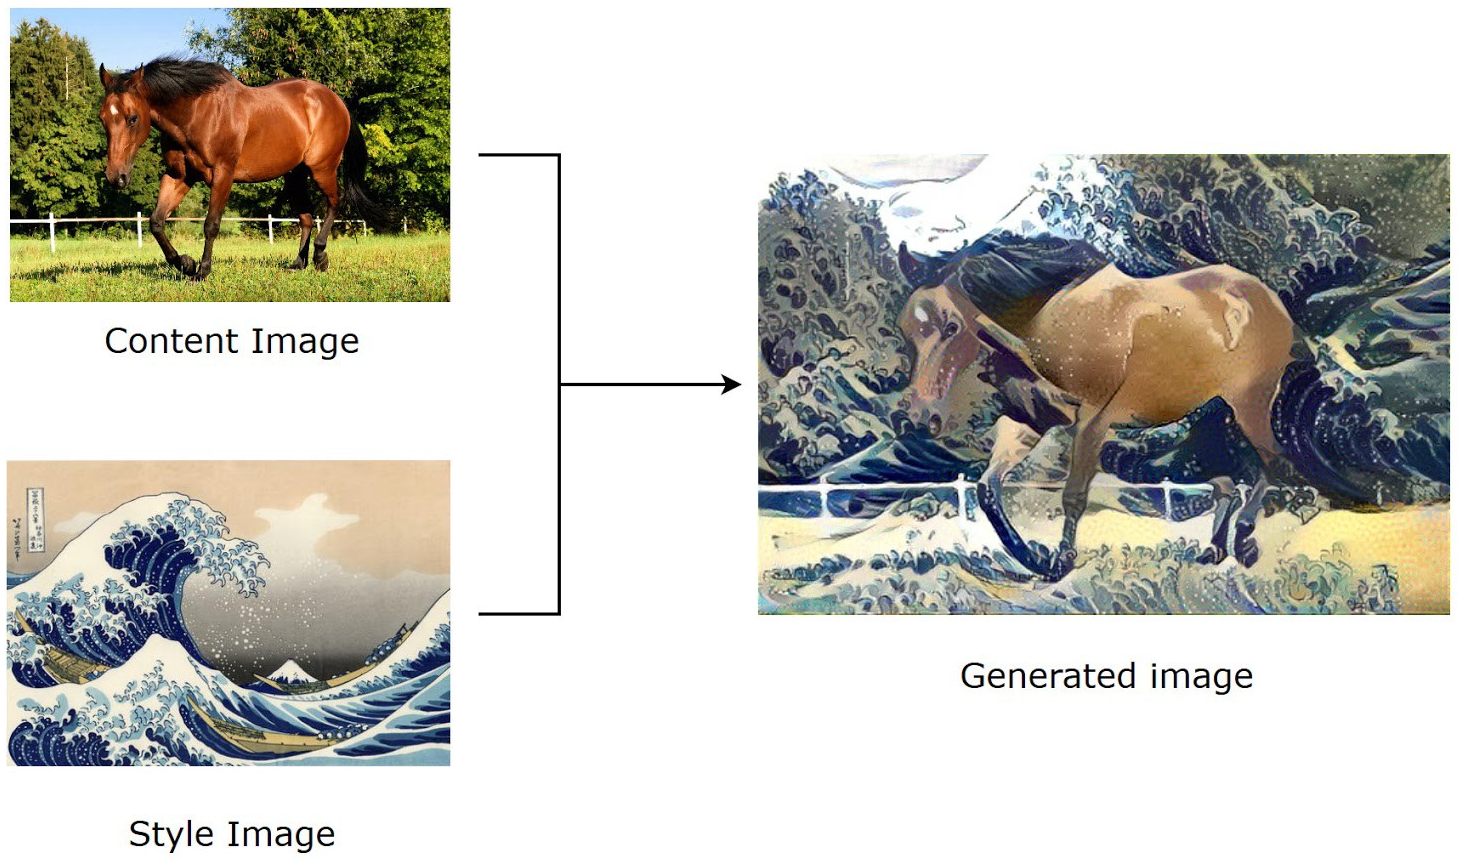
\includegraphics[width=0.45\textwidth]{resources/png/example.png}
        \caption{An example of neural style transfer product \cite{towards-data-science-img}.}
        \label{fig:example}
    \end{figure}
    
    There are several reasons why we chose this task.\\
    
    Firstly, we think that a visual output (or at least an output that can be made visual) was more appealing than a more abstract one. Also, with this kind of task, we will not have to wait hours or close to the end of the project to see if the results are satisfactory or not (unlike with some recurrent neural networks).\\
    
    Secondly, there exists some papers tackling this task on which we can base our work and, among some other project propositions, this was the one Mr Sabatelli advised us to take and was the most enthusiastic about. So we have a lot of resources at our disposal.\\
    
    Finally, we believe satisfactory results can be obtained with the limited time we will have to dedicate to this project. Indeed, in view of our still weak knowledge in the field and the other projects we must work on in parallel, we preferred to choose a project where we will be able to achieve results and present a complete and accomplished work within the allotted time.\\
    
    %%%%%%%%%%%%%%%%%%%%
    %%%%%%%%%%%%%%%%%%%%
    %%%%%%%%%%%%%%%%%%%%
    
    % ----- Related work ----- %
    
    % TO DO
    % -----
    % Research that is related to the considered problem
    
    \section{Related work}
    
    Once we had decided to tackle this task, we looked in the literature for papers or links concerning this problem and found some from which we will take inspiration and/or will try to recreate and retrain the models. These sources, as of today, are the following : \\
    
    \cite{1508-06576} : a paper written by Leon A. Gatys, Alexander S. Ecker and Matthias Bethge which seems to be the original paper for the task of neural style transfer. Its sets the base for the task.\\
    
    \cite{github-neural-style-transfer} : a Github repository implementing the paper cited just above.\\
    
    \cite{tensorflow-style-transfer} : a Tensorflow tutorial about neural style transfer.\\
    
    \cite{1705-04058} : this paper provides an overview of the current progress towards NST and a comparison between the approaches. This paper can serve as a starting point to choose the algorithm we will implement and to provide ideas for improvements.
    
    %%%%%%%%%%%%%%%%%%%%
    %%%%%%%%%%%%%%%%%%%%
    %%%%%%%%%%%%%%%%%%%%
    
    % ----- Methods ----- %
    
    % TO DO
    % -----
    % A clear and detailed description of the neural networks (architecture, training-parameters, loss function, data)
    
    \section{Methods}
    
    to do
    
    %%%%%%%%%%%%%%%%%%%%
    %%%%%%%%%%%%%%%%%%%%
    %%%%%%%%%%%%%%%%%%%%
    
    % ----- Results ----- %
    
    % TO DO
    % -----
    % Qualitative analysis : could include examples of generated images, correct vs wrong predictions, ...
    % Quantitative analysis : general overview of final performance, loss curves, comparison table with error-bars, ...
    
    \section{Results}
    
    to do
    
    %%%%%%%%%%%%%%%%%%%%
    %%%%%%%%%%%%%%%%%%%%
    %%%%%%%%%%%%%%%%%%%%
    
    % ----- Discussion ----- %
    
    % TO DO
    % -----
    % A critical discussion of the performance of the neural network, analysis of the potential limitations, tips for future work
    
    \section{Discussion}
    
    to do
    
    %%%%%%%%%%%%%%%%%%%%
    %%%%%%%%%%%%%%%%%%%%
    %%%%%%%%%%%%%%%%%%%%
    
    % ----- References ----- %
    
    \bibliographystyle{unsrt}
    \bibliography{references.bib}
    \nocite{*}
\end{document}
